% Provenance (never printed): cycle 2 "Questionner le monde" (states of water in
% weather phenomena; daily observation), see sources/book1/PROVENANCE.md.
% Book 1, grade 1, chapter 1. No real-world number in this chapter.
\chapter{نراقب الطقس}\label{ch:g1:watching-the-weather}

الوقت صباح باكر. تستيقظ لينا، وتصعد على الكرسي قرب نافذة غرفتها
وتنظر إلى الخارج. السماء رمادية. وقطرات ماء صغيرة تسيل على الزجاج.
وسطوح البيوت في الجهة المقابلة من الشارع مبللة لامعة، والشجرة في
الحديقة يقطر منها الماء.

تسأل: «ماذا ألبس اليوم؟»

لا تحتاج لينا إلى كتاب ولا إلى آلة لتجيب. يكفيها أن تنظر من النافذة.
النافذة هي أول محطة أرصاد لها.

\begin{omfigure}
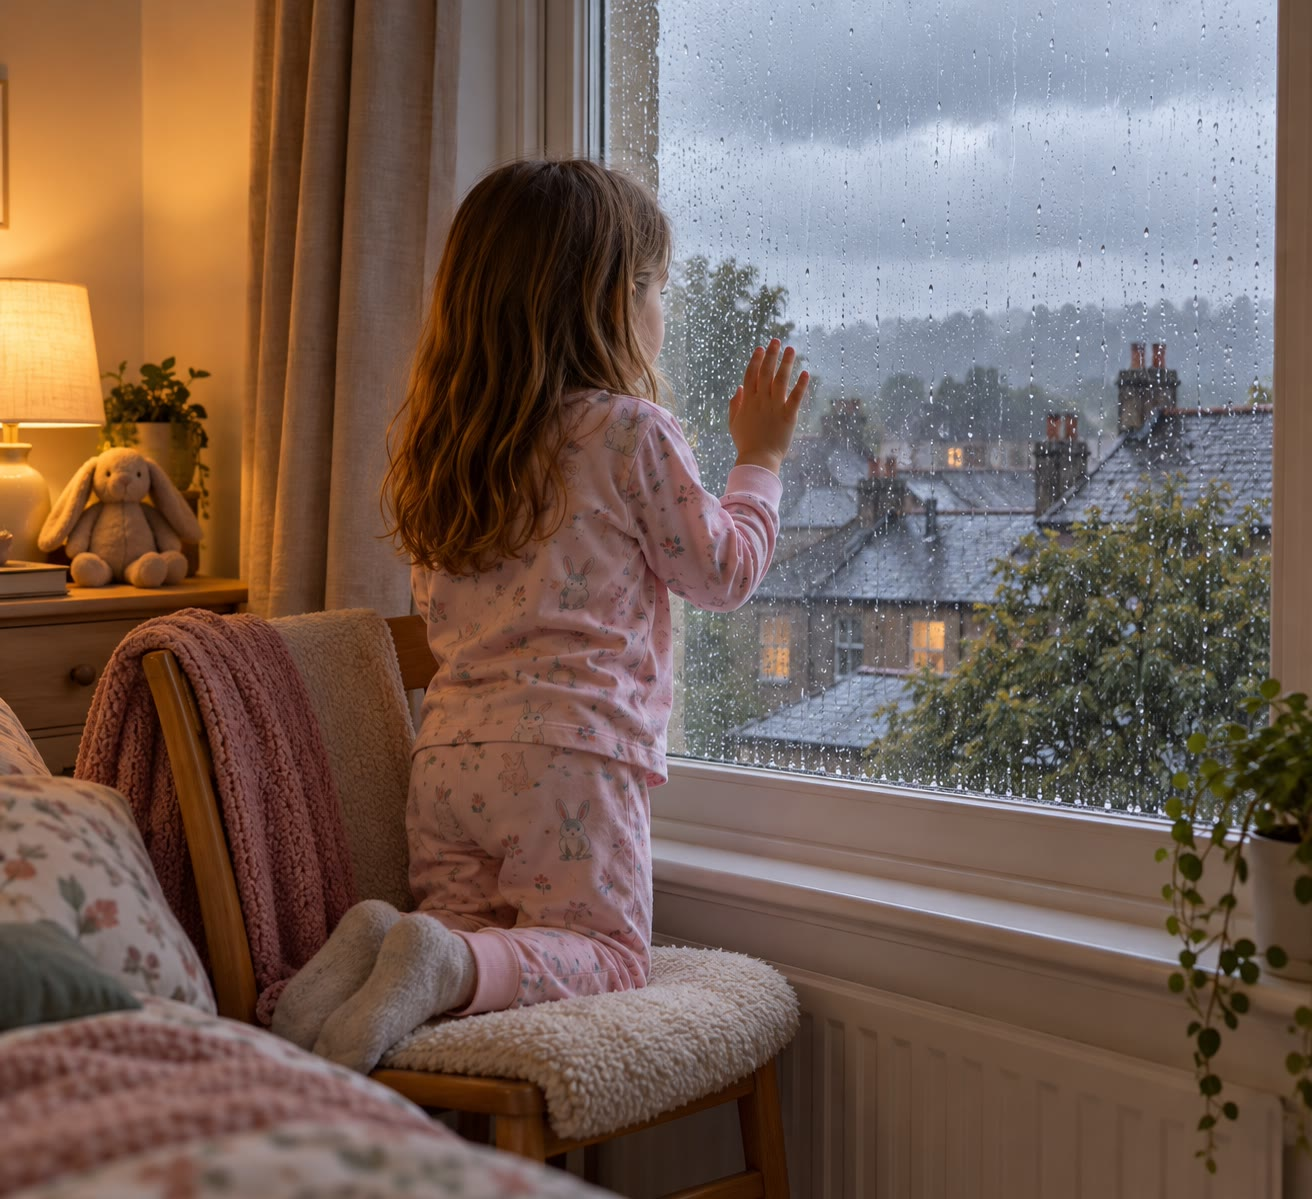
\includegraphics[width=0.72\linewidth]{images/book1/ai/g1-rainy-window.jpg}

{\small صباح رمادي ماطر نراه من خلال نافذة.}
\end{omfigure}

\begin{recall}
كل صباح تشرق الشمس فيبدأ النهار، وكل مساء تغرب فيأتي الليل. وقد رأيت
في كتب الفيزياء لماذا يعقب الليلُ النهارَ. وفي هذا الفصل ننظر إلى شيء
آخر يتغير طوال الوقت: \omterm{def:g1:watching-the-weather:weather}{الطقس}.
\end{recall}

\section{ما الطقس؟}

حين نخرج نحس بالهواء على وجوهنا. قد يكون دافئًا أو باردًا. وقد يكون
ساكنًا، أو يدفع شعرنا وثيابنا: عندئذ تكون هناك ريح. ونرفع أعيننا إلى
السماء. قد تكون زرقاء صافية، أو تغطيها الغيوم. وأحيانًا يسقط المطر من
الغيوم، وأحيانًا الثلج. هذا كله معًا هو \omterm{def:g1:watching-the-weather:weather}{الطقس}.

\begin{definition}[الطقس]\label{def:g1:watching-the-weather:weather}
\emph{الطقس}\index{طقس} هو حال الهواء والسماء في مكان واحد وفي لحظة
واحدة: مشمس أو غائم، جاف أو ماطر أو مثلج، هادئ أو عاصف، دافئ أو
بارد.
\end{definition}

لكي نصف \omterm{def:g1:watching-the-weather:weather}{الطقس} نجيب عن بضعة أسئلة بسيطة:
\begin{enumerate}
  \item \textbf{كيف تبدو السماء؟} أهي زرقاء والشمس مشرقة؟ أفيها
        بضع غيوم، أم أن السماء كلها رمادية؟
  \item \textbf{هل يسقط شيء من السماء؟} مطر؟ ثلج؟ لا شيء؟
  \item \textbf{هل هناك ريح؟} هل تتحرك أوراق الأشجار؟ هل يرفرف
        العلم؟
  \item \textbf{هل الجو دافئ أم بارد؟} هل نحتاج إلى معطف؟
\end{enumerate}

\begin{omfigure}
\begin{minipage}[b]{0.49\linewidth}\centering
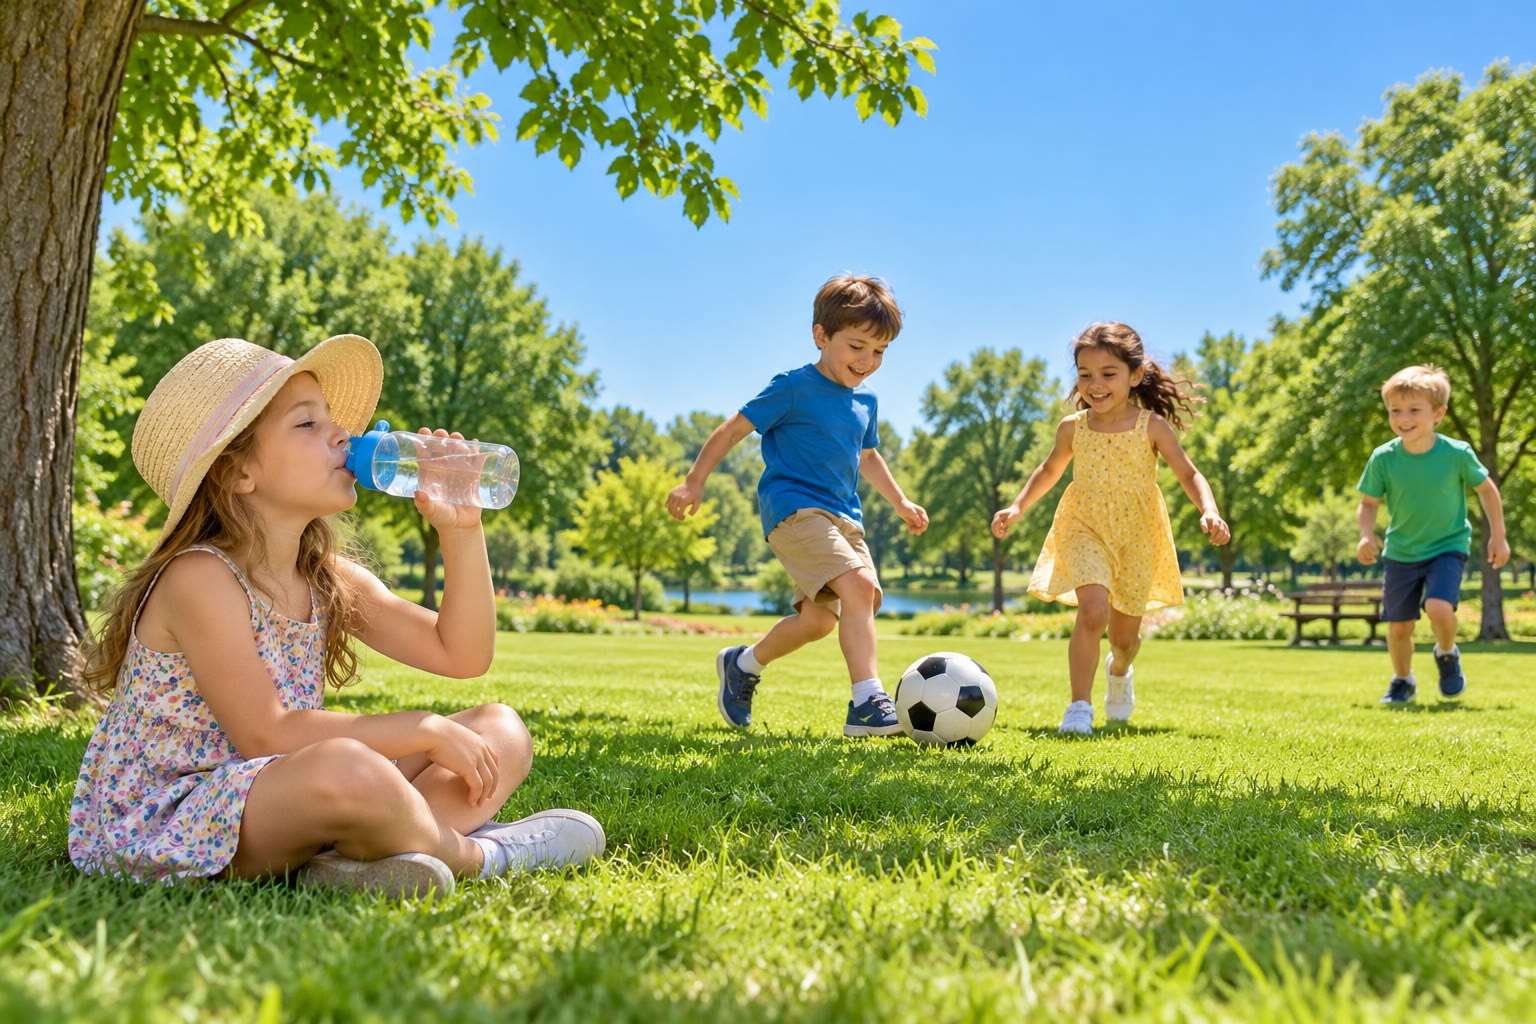
\includegraphics[width=\linewidth]{images/book1/ai/g1-sunny-park.jpg}

{\small مشمس ودافئ.}
\end{minipage}\hfill
\begin{minipage}[b]{0.49\linewidth}\centering
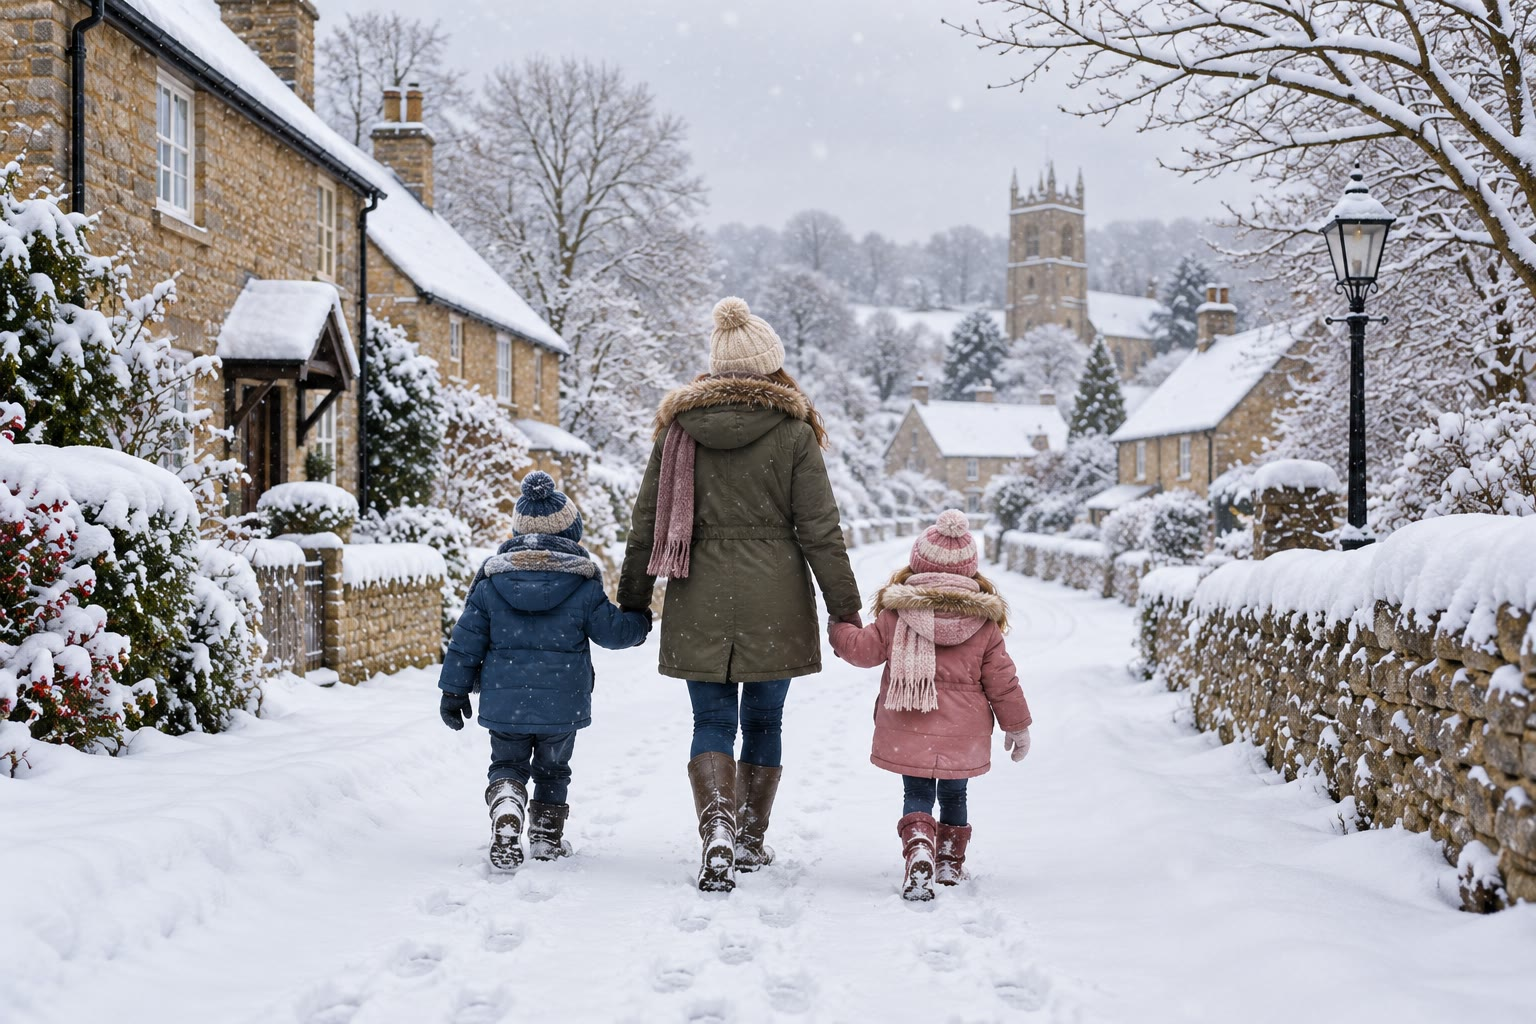
\includegraphics[width=\linewidth]{images/book1/ai/g1-snowy-street.jpg}

{\small مثلج وبارد.}
\end{minipage}

\medskip
\begin{minipage}[b]{0.49\linewidth}\centering
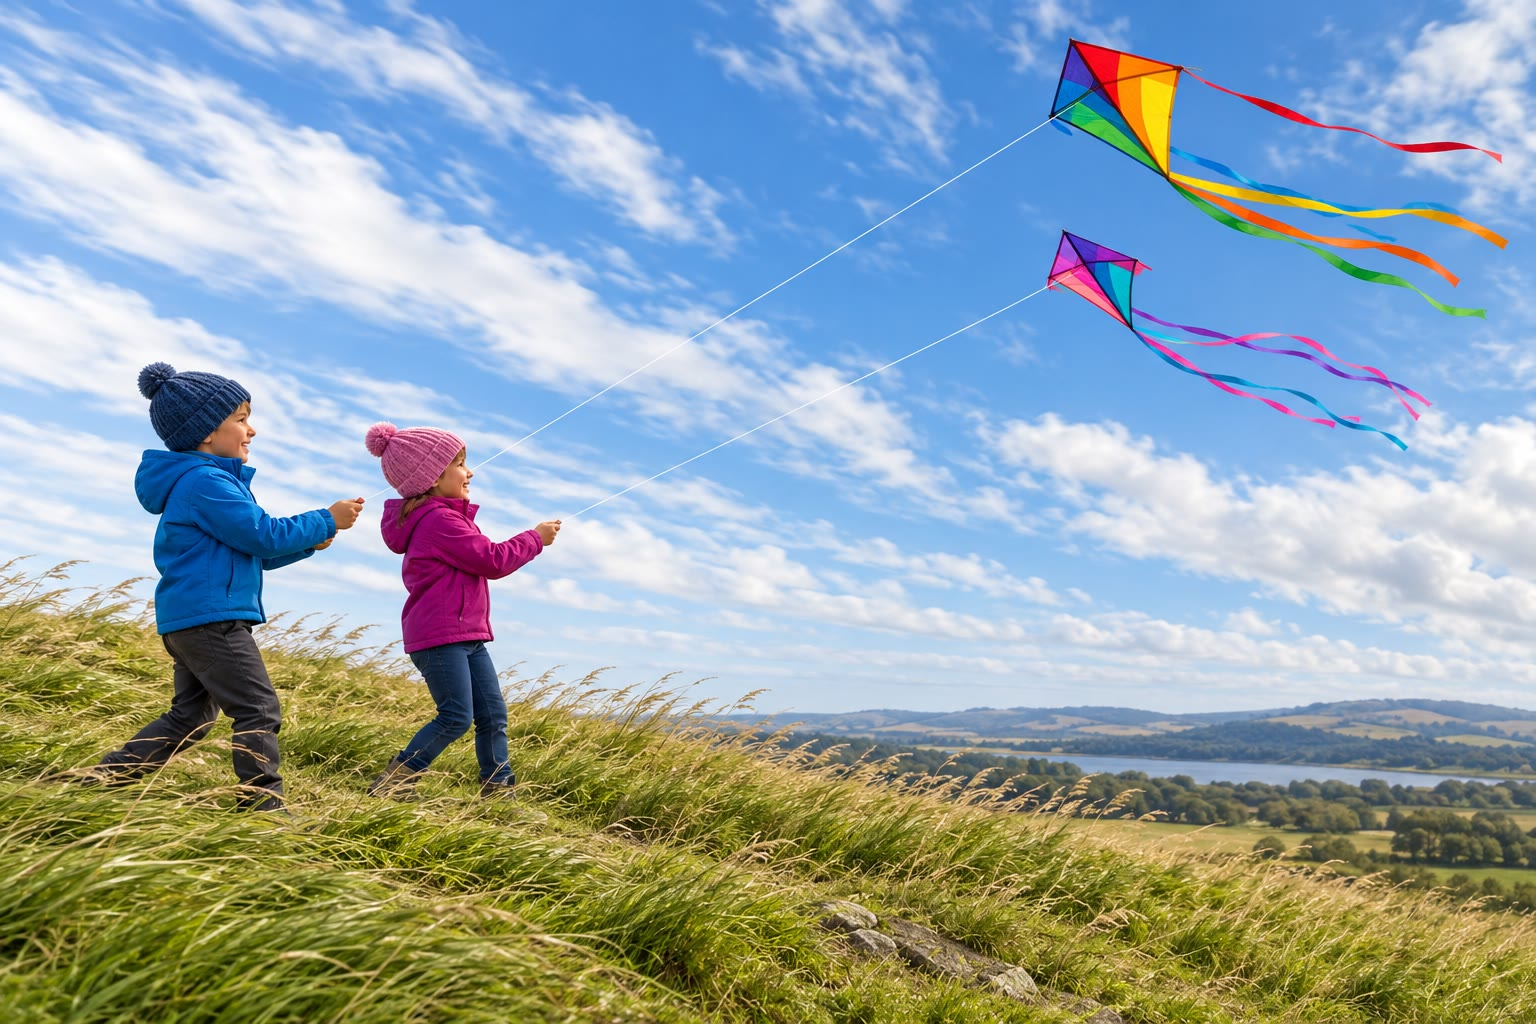
\includegraphics[width=\linewidth]{images/book1/ai/g1-windy-kites.jpg}

{\small عاصف: الطائرات الورقية تطير.}
\end{minipage}\hfill
\begin{minipage}[b]{0.49\linewidth}\centering
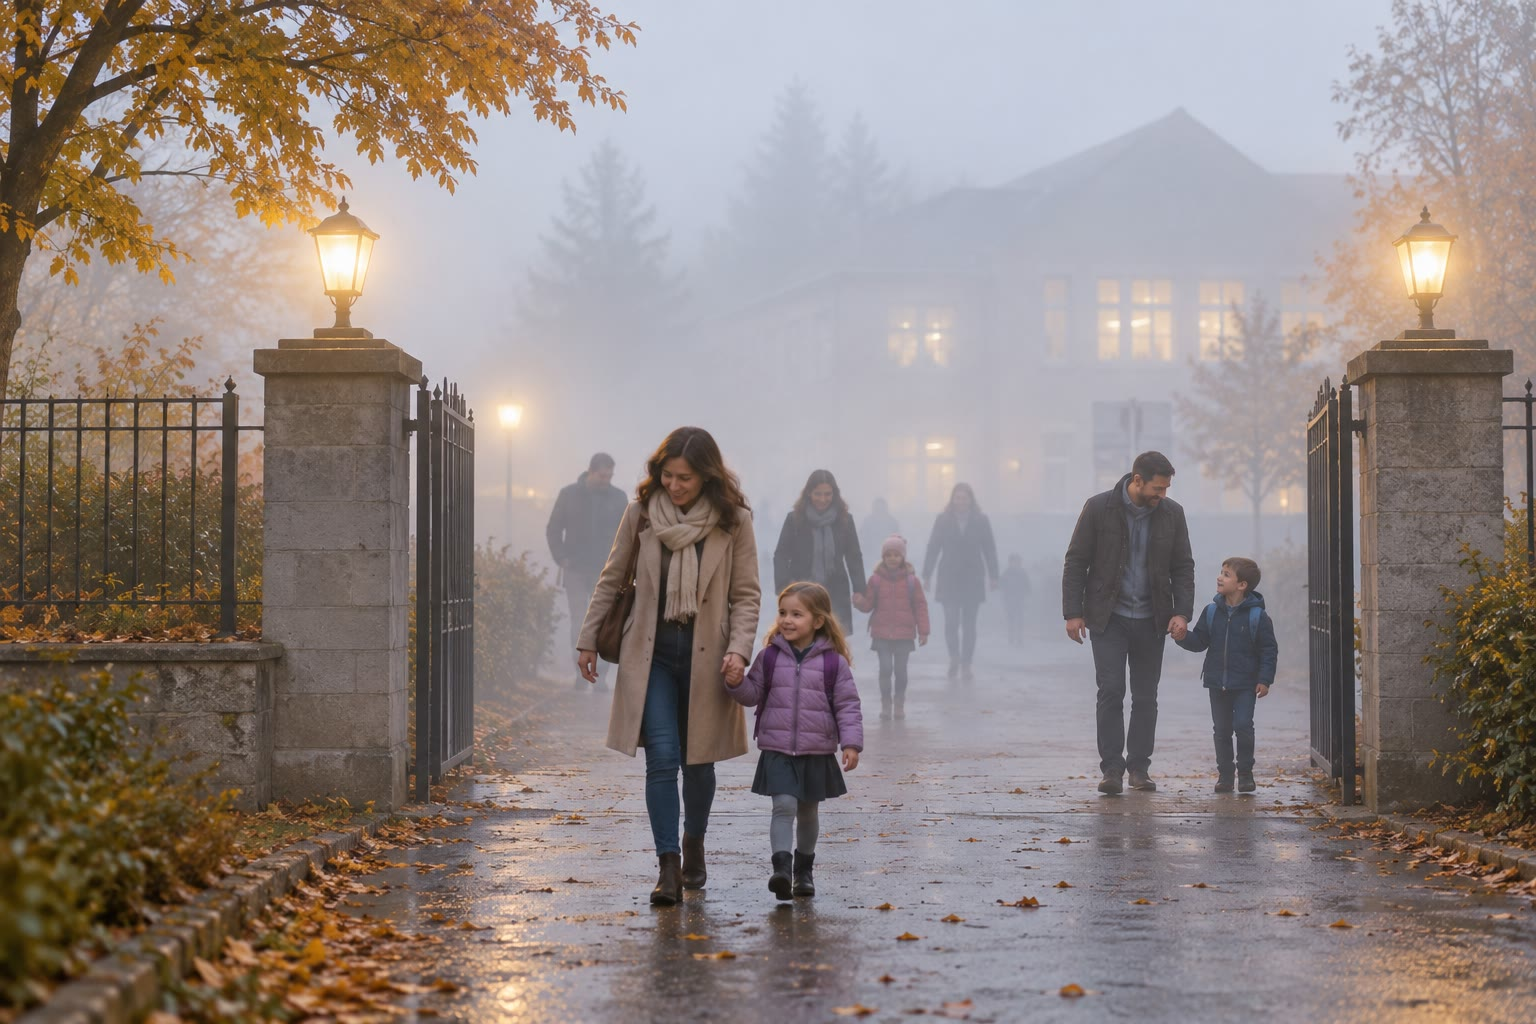
\includegraphics[width=\linewidth]{images/book1/ai/g1-foggy-school.jpg}

{\small ضبابي: لا نرى بعيدًا.}
\end{minipage}
\end{omfigure}

\begin{example}[الضباب]\label{ex:g1:watching-the-weather:fog}
في بعض الصباحات يبدو الهواء نفسه أبيض، وكأن الأشجار في آخر الشارع
تختفي. هذا هو الضباب. الضباب غيمة تلامس الأرض. وحين يدفأ النهار
يزول الضباب في الغالب.
\end{example}

\section{رموز الطقس وجدول الطقس}

وصف \omterm{def:g1:watching-the-weather:weather}{الطقس} بالكلمات يأخذ وقتًا طويلًا. لذلك يستعمل الذين يراقبون \omterm{def:g1:watching-the-weather:weather}{الطقس}
رسومًا صغيرة بدلًا منها: \omterm{def:g1:watching-the-weather:weather-chart}{رموز الطقس}. كل رمز سهل الرسم وسهل التعرف
عليه.

\begin{omfigure}
\begin{tikzpicture}[x=1cm, y=1cm]
  \foreach \i/\n/\t in {0/sun/مشمس, 1/suncloud/شمس وغيوم,
      2/cloud/غائم, 3/rain/ماطر, 4/shower/زخات مطر} {
    \pic[scale=1.25, transform shape] at (\i*2.6,0) {omwx=\n};
    \node[font=\small, align=center, text width=2.4cm] at (\i*2.6,-1.05) {\t};
  }
  \foreach \i/\n/\t in {0/snow/مثلج, 1/storm/عاصفة رعدية, 2/fog/ضبابي,
      3/wind/عاصف} {
    \pic[scale=1.25, transform shape] at (\i*2.6+1.3,-2.6) {omwx=\n};
    \node[font=\small, align=center, text width=2.4cm] at (\i*2.6+1.3,-3.65) {\t};
  }
\end{tikzpicture}

{\small تسعة \omterm{def:g1:watching-the-weather:weather-chart}{رموز للطقس}. للعاصفة الرعدية غيمة داكنة وبرق؛ وزخات المطر
تأتي وبينها فترات مشمسة.}
\end{omfigure}

\begin{definition}[جدول الطقس]\label{def:g1:watching-the-weather:weather-chart}
\emph{رمز الطقس}\index{رمز الطقس} رسم صغير يبين نوعًا واحدًا من \omterm{def:g1:watching-the-weather:weather}{الطقس}.
و\emph{جدول الطقس}\index{جدول الطقس} جدول نكتب فيه، يومًا بعد يوم،
\omterm{def:g1:watching-the-weather:weather}{الطقس} الذي رأيناه، برموز \omterm{def:g1:watching-the-weather:weather}{الطقس}.
\end{definition}

يستطيع الفصل أن يحتفظ \omterm{def:g1:watching-the-weather:weather-chart}{بجدول للطقس} أسبوعًا كاملًا. كل صباح، ثم كل
بعد ظهر، ينظر أحد الأطفال إلى الخارج ويرسم الرمز في الخانة المناسبة.
ونكتب أيضًا هل الجو دافئ أم بارد.

\begin{omfigure}
\begin{tikzpicture}[x=1cm, y=1cm]
  \def\cw{1.9}
  \foreach \d [count=\i from 0] in {الاثنين, الثلاثاء, الأربعاء, الخميس,
      الجمعة, السبت, الأحد}
    \node[font=\scriptsize\bfseries] at ({1.6+\i*\cw+\cw/2},0.35) {\d};
  \node[font=\scriptsize\bfseries, anchor=east] at (1.45,-0.5) {الصباح};
  \node[font=\scriptsize\bfseries, anchor=east] at (1.45,-1.5) {بعد الظهر};
  \node[font=\scriptsize\bfseries, anchor=east, align=right] at (1.45,-2.35) {دافئ أم\\بارد؟};
  \draw[black!60] (1.6,0) rectangle ({1.6+7*\cw},-2.7);
  \foreach \i in {1,...,6}
    \draw[black!60] ({1.6+\i*\cw},0.65) -- ({1.6+\i*\cw},-2.7);
  \draw[black!60] (1.6,0.65) -- ({1.6+7*\cw},0.65);
  \draw[black!60] (1.6,0.65) -- (1.6,0);
  \draw[black!60] ({1.6+7*\cw},0.65) -- ({1.6+7*\cw},0);
  \draw[black!60] (1.6,-1) -- ({1.6+7*\cw},-1);
  \draw[black!60] (1.6,-2) -- ({1.6+7*\cw},-2);
  \foreach \i/\m/\a/\w in {0/rain/rain/بارد, 1/cloud/suncloud/بارد,
      2/sun/sun/دافئ, 3/sun/suncloud/دافئ, 4/suncloud/shower/دافئ,
      5/fog/sun/دافئ, 6/cloud/rain/بارد} {
    \pic[scale=0.8, transform shape] at ({1.6+\i*\cw+\cw/2},-0.5) {omwx=\m};
    \pic[scale=0.8, transform shape] at ({1.6+\i*\cw+\cw/2},-1.5) {omwx=\a};
    \node[font=\scriptsize] at ({1.6+\i*\cw+\cw/2},-2.35) {\w};
  }
\end{tikzpicture}

{\small \omterm{def:g1:watching-the-weather:weather-chart}{جدول الطقس} الذي سجله فصل دراسي خلال أسبوع من الربيع.}
\label{fig:g1:watching-the-weather:chart}
\end{omfigure}

\begin{method}[قراءة جدول الطقس]\label{met:g1:watching-the-weather:read}
لقراءة \omterm{def:g1:watching-the-weather:weather-chart}{جدول الطقس}:
\begin{enumerate}
  \item ابحث عن عمود اليوم الذي تريده؛
  \item انظر إلى الصف: الصباح أو بعد الظهر؛
  \item سمِّ \omterm{def:g1:watching-the-weather:weather}{الطقس} الذي يبينه الرمز.
\end{enumerate}
لكي تعرف كم يومًا كان مشمسًا، مرّر إصبعك على طول صف وعُدّ رموز
الشمس.
\end{method}

\begin{example}[قراءة جدول الفصل]\label{ex:g1:watching-the-weather:read}
في جدول هذا الفصل، كان صباح الاثنين ماطرًا باردًا. ويوم الأربعاء كان
مشمسًا طوال النهار. ويوم السبت انقشع ضباب الصباح وحلت محله الشمس بعد
الظهر. وفي صباحات الأسبوع رسم الفصل الشمس في يومين: الأربعاء
والخميس.
\end{example}

\section{الطقس يتغير}

لا يبقى \omterm{def:g1:watching-the-weather:weather}{الطقس} على حاله. إنه يتغير خلال النهار، ومن يوم إلى اليوم
التالي، وعلى مدار السنة.

\begin{itemize}
  \item \textbf{خلال يوم واحد.} قد يتحول صباح رمادي إلى بعد ظهر مشمس.
        وقد ينتهي صباح أزرق صافٍ بعاصفة. وفي الصباح الباكر وفي الليل
        يكون الجو عادة أبرد منه بعد الظهر.
  \item \textbf{من يوم إلى اليوم التالي.} انظر إلى جدول الفصل: لا يوجد
        يومان في الأسبوع متشابهان تمامًا.
  \item \textbf{على مدار السنة.} في الصيف تكون الأيام عادة دافئة، وفي
        الشتاء تكون عادة باردة؛ وفي أماكن كثيرة لا يسقط الثلج إلا في
        الشتاء. وكتب الفيزياء تشرح لماذا تعود الفصول كل
        سنة.
\end{itemize}

\begin{omfigure}
\begin{tikzpicture}[x=1cm, y=1cm]
  \draw[black!50, line width=0.8pt, -{Stealth[length=2.5mm]}] (0,0) -- (12.2,0);
  \foreach \x/\n/\t/\h in {0.9/fog/الصباح الباكر/منعش, 3.5/suncloud/الصباح/معتدل,
      6.1/sun/بعد الظهر/دافئ, 8.7/storm/آخر النهار/دافئ وعاصف,
      11.2/suncloud/المساء/أبرد} {
    \pic[scale=1.1, transform shape] at (\x,0.85) {omwx=\n};
    \fill[black!60] (\x,0) circle (1.5pt);
    \node[font=\scriptsize\bfseries, below] at (\x,-0.12) {\t};
    \node[font=\scriptsize, below] at (\x,-0.5) {\h};
  }
\end{tikzpicture}

{\small يوم صيفي من الصباح إلى المساء: \omterm{def:g1:watching-the-weather:weather}{الطقس} يتغير خمس
مرات.}
\label{fig:g1:watching-the-weather:day}
\end{omfigure}

\begin{omfigure}
\begin{tikzpicture}[x=1cm, y=1cm]
  \foreach \i/\s/\c/\g/\w/\gr in {0/الربيع/green!55!black/pink!60/suncloud/green!35,
      1/الصيف/green!45!black/green!50!black/sun/green!35,
      2/الخريف/orange!80!black/orange!70/rain/green!25!brown!30,
      3/الشتاء/black!55/white/snow/white} {
    \begin{scope}[shift={(\i*3.15,0)}]
      \draw[black!30, rounded corners=3pt, fill=ocBlue!6] (-1.4,-0.45) rectangle (1.4,3.05);
      \fill[\gr] (-1.4,-0.45) rectangle (1.4,0);
      \draw[black!25] (-1.4,0) -- (1.4,0);
      \fill[brown!60!black] (-0.09,0) rectangle (0.09,1.0);
      \draw[brown!60!black, line width=1.6pt] (0,0.75) -- (-0.5,1.35);
      \draw[brown!60!black, line width=1.6pt] (0,0.9) -- (0.45,1.45);
      \ifnum\i<3
        \fill[\c, opacity=0.85] (0,1.55) circle (0.72);
        \ifnum\i=0 \foreach \a in {20,80,140,200,260,320} \fill[\g] (0,1.55) ++(\a:0.45) circle (0.09); \fi
        \ifnum\i=2 \foreach \x/\y in {-0.9/0.15,0.7/0.3,0.95/0.1} \fill[\g] (\x,\y) circle (0.07); \fi
      \else
        \draw[white, line width=2.4pt] (-0.5,1.35) -- (-0.35,1.17);
        \draw[white, line width=2.4pt] (0.45,1.45) -- (0.3,1.27);
      \fi
      \pic[scale=0.8, transform shape] at (0.95,2.55) {omwx=\w};
      \node[font=\small\bfseries] at (0,-0.75) {\s};
    \end{scope}
  }
\end{tikzpicture}

{\small الشجرة نفسها في الفصول الأربعة: أزهار في الربيع، وأوراق خضراء
كثيفة في الصيف، وأوراق برتقالية تتساقط في الخريف، وأغصان عارية عليها
الثلج في الشتاء.}
\label{fig:g1:watching-the-weather:seasons}
\end{omfigure}

\begin{remark}[من أين تأتي الريح]\label{rem:g1:watching-the-weather:wind}
لا نستطيع أن نرى الريح، لكننا نرى ما تفعله. العلم وكُمّ الرياح ودخان
المدخنة كلها تدفعها الريح: فهي تشير إلى حيث تذهب الريح، إذن تأتي الريح
من الجهة الأخرى.
\end{remark}

\begin{omfigure}
\begin{tikzpicture}[x=1cm, y=1cm]
  % ground
  \fill[green!30!omLithAlluv] (-0.4,-0.1) rectangle (8.4,0);
  % windsock on a pole
  \draw[black!70, line width=1.2pt] (1,0) -- (1,3.2);
  \fill[orange!85, draw=black!60] (1,3.15) -- (3.4,2.95) -- (3.4,2.55) -- (1,2.45) -- cycle;
  \fill[white] (1.6,3.1) -- (2.2,3.05) -- (2.2,2.5) -- (1.6,2.47) -- cycle;
  \fill[white] (2.8,3.0) -- (3.4,2.95) -- (3.4,2.55) -- (2.8,2.53) -- cycle;
  \draw[black!60] (1,3.15) -- (3.4,2.95) -- (3.4,2.55) -- (1,2.45);
  % flag
  \draw[black!70, line width=1.2pt] (5.4,0) -- (5.4,3.2);
  \fill[ocBlue!70, draw=black!60] (5.4,3.15) .. controls (6.0,3.3) and (6.4,2.9) .. (7.1,3.05)
     -- (7.1,2.35) .. controls (6.4,2.2) and (6.0,2.6) .. (5.4,2.45) -- cycle;
  % wind arrows
  \foreach \y in {1.0,1.6}
    \draw[omWxRain, line width=1.4pt, -{Stealth[length=3mm]}] (-0.3,\y) -- (0.7,\y);
  \node[font=\small, align=right, anchor=east] at (-0.45,1.3) {الريح تأتي\\من هنا};
  \draw[black!60, -{Stealth[length=2mm]}] (4.1,2.75) -- (4.9,2.75);
  \node[font=\small, align=left, anchor=west] at (7.5,2.7) {العلم وكُمّ الرياح\\يشيران إلى حيث\\تذهب الريح};
\end{tikzpicture}

{\small كُمّ الرياح وعلم في يوم عاصف. الريح تهب من اليسار
إلى اليمين.}
\end{omfigure}

\section{لماذا نراقب الطقس؟}

كثير من الناس يحتاجون إلى معرفة \omterm{def:g1:watching-the-weather:weather}{الطقس} القادم.
\begin{itemize}
  \item \textbf{المزارعون} يراقبون السماء قبل أن يحصدوا التبن: فالمطر
        يفسده. وفي الربيع يخشون ليلة صقيع قد تقتل النباتات
        الصغيرة.
  \item \textbf{البحارة والصيادون} يراقبون الريح: فالريح القوية تصنع
        أمواجًا كبيرة، فتبقى القوارب في الميناء.
  \item \textbf{الطيارون} يحتاجون إلى معرفة الضباب والعواصف والريح قبل
        أن تقلع الطائرة.
  \item \textbf{الفصل} الذي يخرج في نزهة إلى الغابة يريد أن يعرف أيأخذ
        معاطف المطر أم قبعات الشمس.
\end{itemize}
وكل يوم يراقب أناس يسمَّون خبراء الأرصاد الجوية الطقسَ في العالم كله،
ويخبروننا، في المذياع أو التلفاز أو الهاتف، كيف سيكون \omterm{def:g1:watching-the-weather:weather}{الطقس} على
الأرجح في الأيام القادمة.

\begin{example}[علامات في السماء]\label{ex:g1:watching-the-weather:signs}
قبل المذياع والهاتف بزمن طويل تعلم الناس قراءة السماء. حين تكبر غيوم
بيضاء صغيرة، بعد الظهر، فتصير أبراجًا عالية داكنة، فهذا يعني أن زخة
مطر أو عاصفة رعدية قادمة. وحين تغير الريح اتجاهها وتمتلئ السماء ببطء
بغلالة رمادية، فكثيرًا ما يأتي المطر بعد بضع ساعات. هذه العلامات لا
تصدق دائمًا، لكنها مفيدة في كثير من الأحيان.
\end{example}

\section{نلبس ما يناسب الطقس}

الآن تستطيع لينا أن تجيب عن سؤالها. السماء تمطر والجو بارد، فستلبس
معطف المطر والحذاء الطويل. وغدًا قد يكون \omterm{def:g1:watching-the-weather:weather}{الطقس} مختلفًا، فتختار من
جديد.

\begin{omfigure}
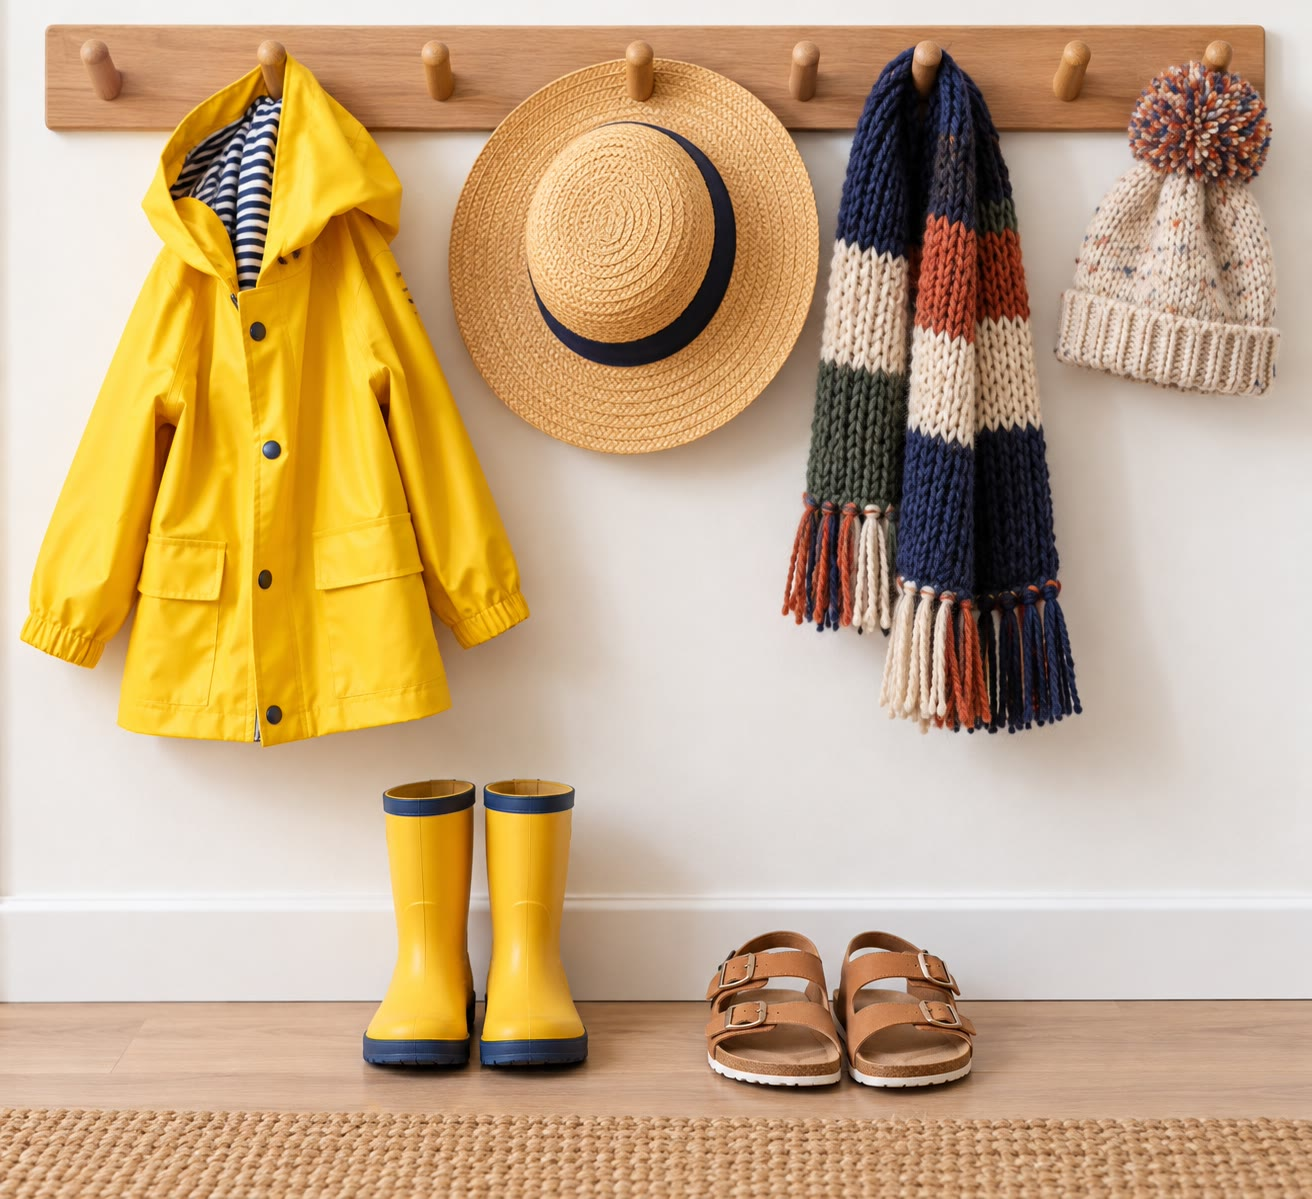
\includegraphics[width=0.66\linewidth]{images/book1/ai/g1-coat-pegs.jpg}

{\small ثياب لكل نوع من \omterm{def:g1:watching-the-weather:weather}{الطقس}: معطف مطر، وقبعة شمس، ووشاح وقبعة
دافئة، وحذاء طويل وصندل.}
\end{omfigure}

\begin{method}[اختيار الثياب المناسبة للطقس]\label{met:g1:watching-the-weather:clothes}
انظر إلى السماء وتحسس الهواء، ثم:
\begin{itemize}
  \item مطر أو زخات: معطف مطر أو مظلة، وحذاء طويل؛
  \item برد أو ثلج: معطف دافئ ووشاح وقبعة وقفازان؛
  \item شمس قوية وحر: قبعة شمس وثياب خفيفة وماء
        للشرب؛
  \item ريح: معطف يُغلق جيدًا؛ والمظلة لا تنفع كثيرًا.
\end{itemize}
\end{method}

\begin{safety}
\textbf{لا تنظر أبدًا إلى الشمس مباشرة}، ولا للحظة واحدة، ولا من خلال
نظارة أو منظار أو آلة تصوير: فقد تؤذي عينيك إلى الأبد. وحين تكون هناك
عاصفة رعدية، ابقَ داخل البيت أو في سيارة، وابتعد عن الأشجار العالية
وعن الماء، وانتظر حتى تمر العاصفة.
\end{safety}

\section{تمارين}

\begin{exercise}[$\star$]\label{exo:g1:watching-the-weather:1}
ارسم رمز كل نوع من \omterm{def:g1:watching-the-weather:weather}{الطقس}: مشمس؛ ماطر؛ مثلج؛ غائم.
\end{exercise}

\begin{exercise}[$\star$]\label{exo:g1:watching-the-weather:2}
كيف \omterm{def:g1:watching-the-weather:weather}{الطقس} في كل صورة من الصور الأربع في القسم «ما \omterm{def:g1:watching-the-weather:weather}{الطقس}؟»؟ استعمل
كلمة أو كلمتين لكل صورة.
\end{exercise}

\begin{exercise}[$\star$]\label{exo:g1:watching-the-weather:3}
انظر إلى \omterm{def:g1:watching-the-weather:weather-chart}{جدول طقس} الفصل. كيف كان \omterm{def:g1:watching-the-weather:weather}{الطقس} صباح الثلاثاء؟ وبعد ظهر
الجمعة؟ وبعد ظهر الأحد؟
\end{exercise}

\begin{exercise}[$\star$]\label{exo:g1:watching-the-weather:4}
في \omterm{def:g1:watching-the-weather:weather-chart}{جدول طقس} الفصل، في أي يوم كان الجو مشمسًا في الصباح وبعد
الظهر؟
\end{exercise}

\begin{exercise}[$\star$]\label{exo:g1:watching-the-weather:5}
صِل كل قطعة ثياب \omterm{def:g1:watching-the-weather:weather}{بطقس}: قبعة شمس؛ حذاء طويل ومعطف مطر؛ وشاح
وقفازان. وأنواع \omterm{def:g1:watching-the-weather:weather}{الطقس} هي: بارد ومثلج؛ حار ومشمس؛
ماطر.
\end{exercise}

\begin{exercise}[$\star$]\label{exo:g1:watching-the-weather:6}
تقول لينا: «انظر، العلم يرفرف!» ما نوع \omterm{def:g1:watching-the-weather:weather}{الطقس}؟
\end{exercise}

\begin{exercise}[$\star$]\label{exo:g1:watching-the-weather:7}
صحيح أم خطأ؟ اشرح.
\begin{enumerate}
  \item \omterm{def:g1:watching-the-weather:weather}{الطقس} دائمًا هو نفسه في الصباح وبعد الظهر.
  \item الضباب غيمة تلامس الأرض.
  \item القاعدة «لا تنظر أبدًا إلى الشمس، ولا بعين واحدة» قاعدة جيدة.
\end{enumerate}
\end{exercise}

\begin{exercise}[$\star\star$]\label{exo:g1:watching-the-weather:8}
في \omterm{def:g1:watching-the-weather:weather-chart}{جدول طقس} الفصل، عُدّ فترات بعد الظهر التي فيها مطر أو زخات. وعُدّ
الأيام الباردة. هل كان الأسبوع دافئًا في أغلبه أم باردًا في أغلبه؟
\end{exercise}

\begin{exercise}[$\star\star$]\label{exo:g1:watching-the-weather:9}
هذا ما رآه سام من نافذته خلال يوم واحد: في الصباح سماء رمادية؛ وعند
الغداء قطرات على النافذة؛ وفي المساء سماء زرقاء فيها بضع غيوم. ارسم
\omterm{def:g1:watching-the-weather:weather-chart}{رموز الطقس} الثلاثة بالترتيب الصحيح.
\end{exercise}

\begin{exercise}[$\star\star$]\label{exo:g1:watching-the-weather:10}
في صورة كُمّ الرياح والعلم، تأتي الريح من اليسار. وفي يوم آخر يشير
علم إلى اليسار. من أي جهة تأتي الريح في ذلك
اليوم؟
\end{exercise}

\begin{exercise}[$\star\star$]\label{exo:g1:watching-the-weather:11}
انظر إلى رسم الشجرة نفسها في الفصول الأربعة. في أي فصل لا تكون على
الشجرة أوراق؟ وفي أي فصل تكون عليها أزهار؟ وأي \omterm{def:g1:watching-the-weather:weather-chart}{رمز طقس} رُسم للشتاء،
ولماذا يناسب ذلك الفصل؟
\end{exercise}
